\documentclass{article}
\usepackage{graphicx} % Required for inserting images
\usepackage{amsmath} 
\usepackage{listings}
\usepackage{xcolor}
\usepackage{float}

\lstset{ 
  language=Python,                % El lenguaje del código
  basicstyle=\ttfamily\footnotesize, % Estilo básico del texto
  keywordstyle=\color{blue},    % Color para palabras clave
  commentstyle=\color{green},   % Color para comentarios
  stringstyle=\color{red},      % Color para strings
  numbers=left,                 % Números de línea a la izquierda
  numberstyle=\tiny\color{gray},% Estilo de los números de línea
  stepnumber=1,                 % Números de línea en cada línea
  numbersep=5pt,                % Separación entre números de línea y código
  backgroundcolor=\color{white},% Color de fondo
  showspaces=false,             % No mostrar espacios
  showstringspaces=false,       % No mostrar espacios en strings
  showtabs=false,               % No mostrar tabs
  frame=single,                 % Cuadro alrededor del código
  tabsize=2,                    % Tamaño de tabulación
  captionpos=b,                 % Título debajo del código
  breaklines=true,              % Cortar líneas largas
  breakatwhitespace=false,      % Cortar solo en espacios
  escapeinside={\%*}{*)}        % Añadir LaTeX dentro del código
}


\title{Nivel 2 Introduccion a Programacion}
\author{Tomas Rodriguez - 202212868}
\date{February 2022}

\begin{document}
\maketitle
\section{Booleanos y sus Operadores}
Los tipos de dato booleanos se caraterizan por ser representados como un \textit{True} y \textit{False} o en el sistema binario como \(1,0\). Este es solo otro tipo de dato mas, por ende, este tambien posee expresiones, se puede almacenar en variables y posee funciones. 
\subsection{Operadores relacionales}
Son aquellos operadores que relacionan valores, variables, parametros, llamados de funciones u otras expresiones entre si. 
\begin{figure}[H]
    \centering
    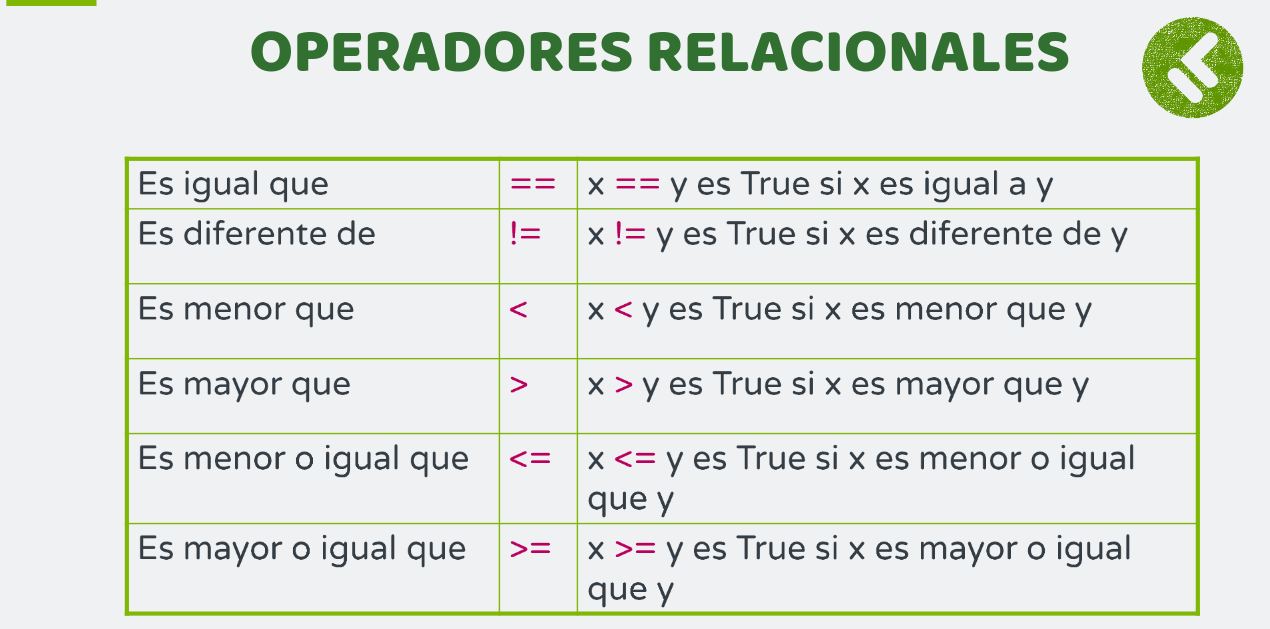
\includegraphics[width=1\linewidth]{OperadoresRelacionales.png}
    \caption{Operadores Relacionales}
    \label{fig:enter-label}
\end{figure}
Existen en python tambien otros operadores, los \textbf{operadores de identidad}.
\begin{itemize}
    \item \textbf{is} y \textbf{is not}: sirven para saber si son iguales o son el mismo, ademas en OOP tienen muchos usos. 
\end{itemize}
\subsection{Operadores logicos}
Permiten describir situaciones mas complejas que los racionales y se dan con valores, variables, parametros, llamados de funciones de retorno booleano.
\begin{figure}[H]
    \centering
    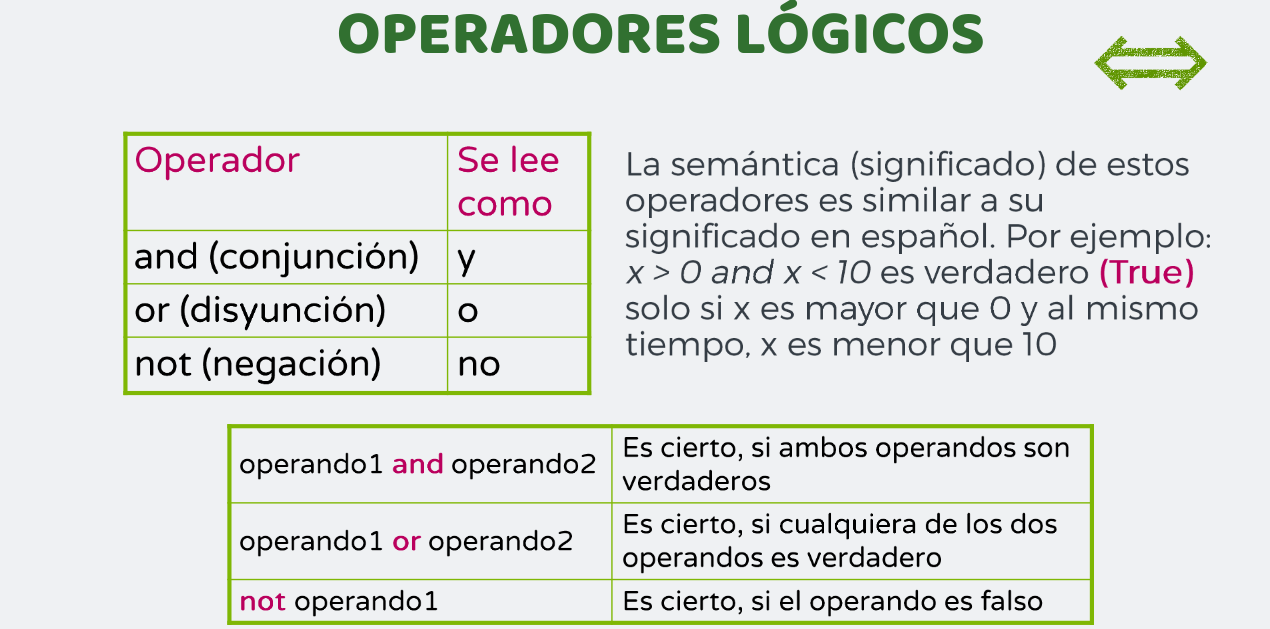
\includegraphics[width=1\linewidth]{OperadoresLogicos.png}
    \caption{Operadores Logicos}
    \label{fig:enter-label}
\end{figure}
\section{Tablas de Verdad y Algebra Booleana}
Las tablas de verdad son aquellas que nos permiten conocer el resultado entre dos operandos entre los operadores logicos posibles.
\begin{table}[H]
    \centering
    \begin{tabular}{ccc}
        a & b & a and b\\
        True & True & True\\
        True & False & False\\
        False & False & False\\
        False & True & False\\
    \end{tabular}
    \caption{Tabla Verdad AND}
    \label{tab:my_label}
\end{table}
\begin{table}[H]
    \centering
    \begin{tabular}{ccc}
        a & b & a or b\\
        True & True & True\\
        True & False & True\\
        False & False & False\\
        False & True & True\\
    \end{tabular}
    \caption{Tabla Verdad OR}
    \label{tab:my_label}
\end{table}
\begin{table}[H]
    \centering
    \begin{tabular}{cc}
        a & Not a\\
        True & False\\
        False & True\\
    \end{tabular}
    \caption{Caption}
    \label{tab:my_label}
\end{table}
Ahora bien, el algebra booleana es un conjunto de reglas que se usa para simplificar las expresiones.
\begin{figure}[H]
    \centering
    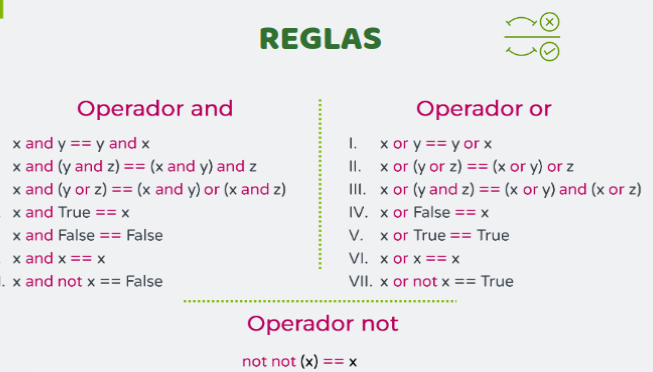
\includegraphics[width=1\linewidth]{ReglasAlgebraBooleana.png}
    \caption{Reglas Algebra Boolena}
    \label{fig:enter-label}
\end{figure}
\section{Condicionales}
Se usan cuando se debe tomar una desicion teniendo en cuenta diferentes casos y de acuerdo a estos la desicion es diferente.
\begin{lstlisting}[language=Python, caption=Operaciones If-else]
if ExpresionBooleana:
    bloque de codigo
else:
    bloque de codigo
\end{lstlisting}
\begin{lstlisting}[language=Python, caption=Operaciones If]
if ExpresionBooleana:
    bloque de codigo
\end{lstlisting}
\begin{lstlisting}[language=Python, caption=Operaciones If en casacada]
if ExpresionBooleana:
    bloque de codigo
elif ExpresionBooleana2:
    bloque de codigo
else:
    bloque de codigo
\end{lstlisting}
\begin{lstlisting}[language=Python, caption=Operaciones If en consecutivo]
if ExpresionBooleana:
    bloque de codigo
if ExpresionBooleana2:
    bloque de codigo
if ExpresionBooleana3:
    bloque de codigo
\end{lstlisting}
\begin{lstlisting}[language=Python, caption=Operaciones If en anidadas]
if ExpresionBooleana:
    bloque de codigo
    if ExpresionBooleana2:
        bloque de codigo
        if ExpresionBooleana3:
            bloque de codigo
\end{lstlisting}
En estas operaciones es bueno tener en cuenta los opuestos logicos de las operaciones logicas.
\begin{figure}[H]
    \centering
    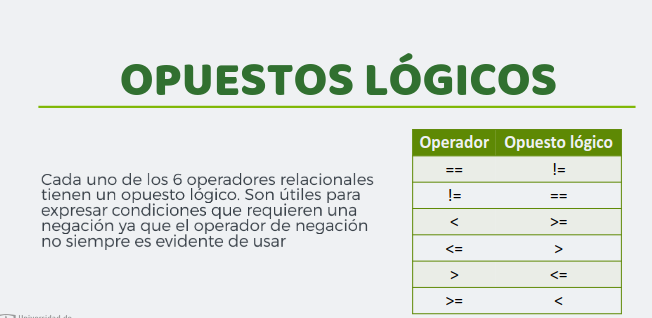
\includegraphics[width=1\linewidth]{OpuestosLogicos.png}
    \caption{Opuestos Logicos}
    \label{fig:enter-label}
\end{figure}
\section{Cadenas de caracteres o Strings}
Existen diversos estandares de caracteres, sin embargo, los mas relevantes son.
\begin{itemize}
    \item ASCII (127 caracteres)
    \item ISO-8859-1 (Incluye caracteres europeos como los del frances)
    \item UNICODE (Incluye todos los idiomas y emojis)
\end{itemize}
Ahora bien, dentro de los \textbf{strings} hay ciertos caracteres los cuales cumplen funciones de control y longitud.
\subsection{Caracteres de control}
Son caracteres especiales que no tienen representaciones triviales.
\begin{itemize}
    \item $\setminus n$: Cambio de linea
    \item $\setminus t$: Tabulador
    \item $\setminus \setminus$: Barra invertida
\end{itemize}
\subsection{Longitud de cadena}
Es en pocas palabras el numero de caracteres o letras que posee una palabra. Para esta se usa la funcion \textit{len()} en python. Hay que tener en cuenta que esta funcion tambien cuenta los espacion entre palabras. 
\subsection{Operaciones}
Asi como en los booleanos y numeros, las cadenas de caracteres tambien pueden ser comparables, por ende, los operadores de relacion y logicos tambien pueden ser aplicados en strings. Sin embargo, en las cadenas hay un nuevo operador.
\begin{itemize}
    \item \textbf{in} y \textbf{not in}: este comprueba si una cadena hace parte de otra cadena. 
\end{itemize}
\begin{lstlisting}[language=Python, caption=Operacion in]
"x" in "manzana" #Va a dar False
"x" not in "manzana" #Va a dar True
\end{lstlisting}
\subsection{Metodos}
Ahora bien, las cadenas tienen sus propios metodos. Sin embargo, hay que tener en cuenta que una vez definida una cadena esta no puede cambiar su contenido, si se quiere cambiar, hay que crear una nueva cadena(\textbf{Inmutabilidad}). Estos son algunos metodos.
\begin{itemize}
    \item lower(): devuelve una nueva cadena con todos los caracteres en minusculas.
    \item upper(): devuelve una nueva cadena con todos los caracteres en mayusculas.
    \item title(): devuelve una nueva cadena con la primera letra de cada palabra en mayusculas.
    \item swapcase(): devuelve una nueva cadena con los caracteres en minuscula convertidos en mayusculas y visceversa.
    \item replace(): Recibe dos cadenas, un patron y un reemplazo, el metodo busca el patron en la cadena y lo cambia por el remplazo en cada una de sus aparciones. 
    \item find(): Se le da una cadena con el fin de que la busque en la cadena principal, esta devuelve el indice en la que se encuentra la cadena en la otra, y si no lo encuentra devuelve \(-1\).
    \item count(): Dada una cadena, cuenta cuantas veces esta esa cadena en la cadena principal.
    \item format(): se colocan \{\} en la cadena con los indices dentro de la forma \{0\} con el fin de que sea remplazado con los parametros del metodo format.
\end{itemize}
Todos estos metodos y su informacion, puede ser consultada con el metodo help() en python.
\section{Diccionarios}
Son \textbf{estructuras de datos}, es decir, tipos de datos compuestos que nos permiten manejar otros datos determinados en \{llave:valor\}. Su tipo de dato en python se determina como \textbf{dict}.\\
Estos se pueden inicar como variable = \{\} y se pueden crear ya con datos. Se pueden agregar datos de la siguente manera:
\begin{lstlisting}[language=Python, caption=Operacion adicion diccionario]
agenda_dia = {}

agenda_dia[6] = "Empieza el dia"
agenda_dia[8] = "Desayuno con Clara"
agenda_dia[9.5] = "Clase de IP"
agenda_dia[11] = "Clase de calculo"
agenda_dia[13] = "Almuerzo"
agenda_dia[15] = "Natacion"
agenda_dia[16] = "Repaso de quimica"
agenda_dia[19.5] = "Visita a los abuelos"

\end{lstlisting}
Ahora bien, para acceder, modificar se usa la forma: 
\begin{lstlisting}[language=Python, caption=Operacion modificacion y consulta diccionario]
#Modificacion
agenda_dia[6] = "Empieza el noche"
#Consulta
agenda_dia[6]
agenda_dia.get(6,"No hay esa hora en la agenda") # Se le da la llave y un valor si no existe
agenda_dia.get(6,None) # Se da el valor de None tambien ya que este significa ausencia de valor
\end{lstlisting}
Por otra parte, en los diccionarios tambien se hace uso de los operadores \textbf{in} y \textbf{not in} con el fin de conocer si la llave existe en el diccionario y tambien se puede usar la funcion \textbf{len()}.\\
Hay una componente a tener en cuenta en los diccionarios y es que son \textbf{mutables}, esto quiere decir que si hay dos variables apuntando al mismo diccionario, y se modifica alguna de estas, la otra tambien se modifica. Entonces, si queremos conservar el diccionario original, debemos hacer una copia con el metodo \textbf{copy()}
\end{document}
